\documentclass[11pt]{article}

%\usepackage[utf8]{inputenc}
\usepackage[a4paper, margin=1in]{geometry}


\usepackage{graphicx}
\usepackage{float}
\usepackage{xcolor}
\usepackage{enumerate}

\usepackage{amsthm}

\usepackage{natbib}

\usepackage{hyperref}
\usepackage{graphicx}

\usepackage[font=small,labelfont=bf]{caption}

\setlength\parindent{0pt}
\setlength\parskip{5pt}

\usepackage{listings}
\lstset{
basicstyle=\small\ttfamily,
columns=flexible,
breaklines=true,,
stepnumber=1,
}

\definecolor{silver}{gray}{0.9}

\theoremstyle{definition}

\newsavebox\notebox
\newtheorem{mynote}{Note}
\newenvironment{note}%
  {\begin{lrbox}{\notebox}%
   \begin{minipage}{\dimexpr\linewidth-2\fboxsep}
   \begin{mynote}}%
  {\end{mynote}%
   \end{minipage}%
   \end{lrbox}%
   \begin{trivlist}
     \item[]\colorbox{silver}{\usebox\notebox}
   \end{trivlist}}

\newsavebox\examplebox
\newtheorem{myexample}{Example}
\newenvironment{example}%
  {\begin{lrbox}{\examplebox}%
   \begin{minipage}{\dimexpr\linewidth-2\fboxsep}
   \begin{myexample}}%
  {\end{myexample}%
   \end{minipage}%
   \end{lrbox}%
   \begin{trivlist}
     \item[]\colorbox{silver}{\usebox\examplebox}
   \end{trivlist}}


\title{The MobiView graphical user interface}
\author{Magnus Dahler Norling}

\begin{document}

\maketitle

\tableofcontents

\section{Introduction}

MobiView is a graphical user interface that can load any model built using the Mobius dll interface. It is created using the Ultimate++ framework and the ScatterCtrl package (\url{ultimatepp.org}).

This document is a work in progress.

\begin{center}
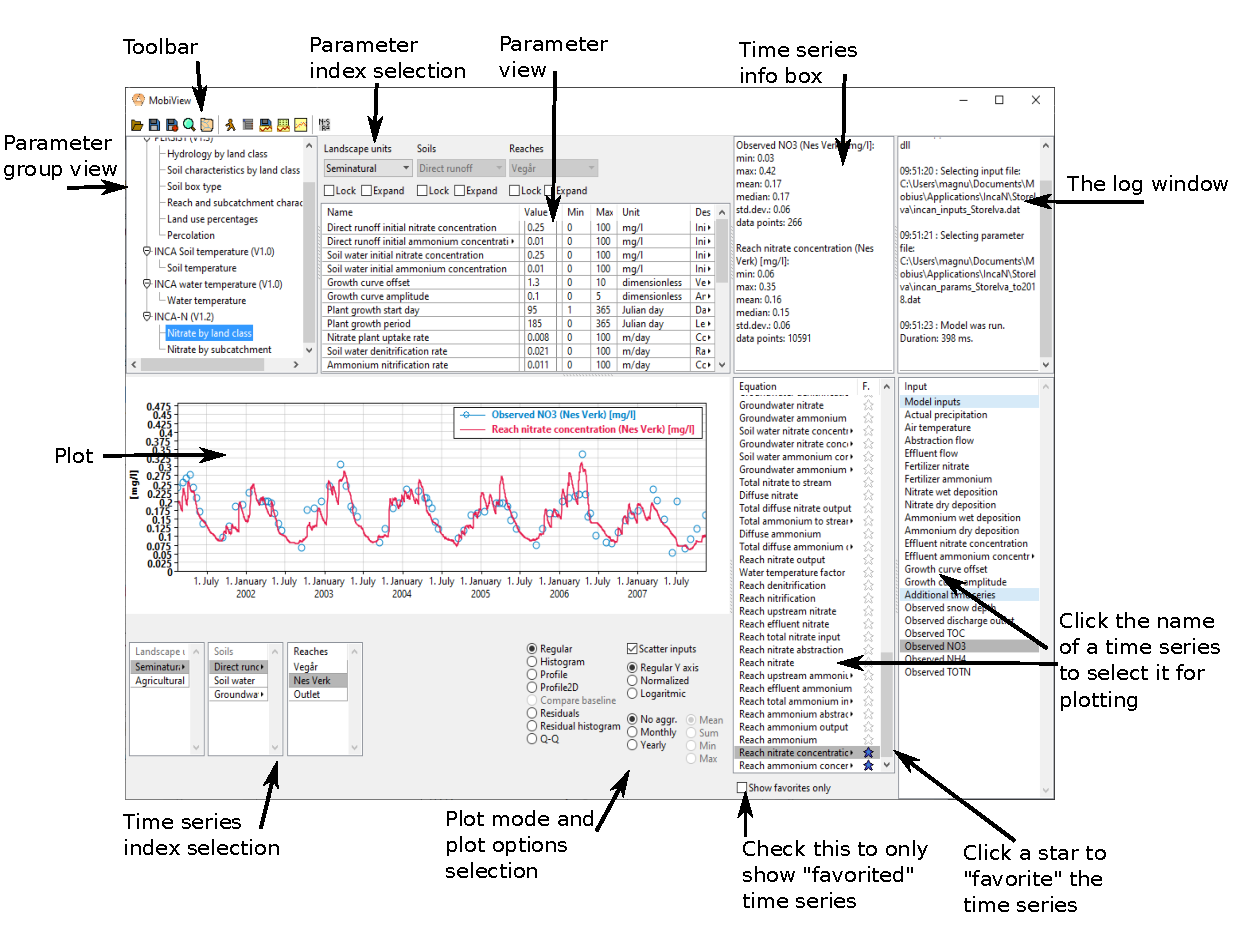
\includegraphics[width=\linewidth]{img/mobiview}
\captionof{figure}{Overview of the MobiView user interface}
\end{center}

\section{The toolbar}

The toolbar has 9 buttons.

\begin{enumerate}
\item Load (ctrl-O). This asks you to select a model dll, an input file, and a parameter file. (On Linux, you load a shared object .so file instead of a dll). The input and parameter files have to be of the .dat format described in the Mobius file format documentation. You can click load even if you have a model and dataset loaded already. This will delete all data from the earlier dataset from memory, so be sure to save any changes you want to keep first.
\item Save parameters (ctrl-S). This saves any edits you have made to the parameters to the current working parameter file (usually the one you loaded).
\item Save parameters as (alt-S). Saves the parameters to a new file. The new file is now the current working file.
\item Search parameters (ctrl-F). Opens a new window that allows you to search for parameters by name. Any matching parameters are displayed in a list, and clicking an item in the list takes you to the right parameter group in the main view. The search is a case-insensitive substring search.
\item Edit indexes (ctrl-E). Opens a new window. You can edit what indexes are in each index set. For non-branched index sets, each index is a line in the text field. If you add a nex index or rename one, the parameters indexed by that index will be given default values. You can also edit the branch connections of branched index sets. The input ids have to be a comma-separated list of numbers of the id's of the input branches to the given branch. In the visualization of the branch connections of the branched index set, no information about actual length or position is used in the visualization, only connectivity.
\item Run model (F7). Runs the model using the parameters that are loaded in the MobiView interface, taking into account any edits. (It does not matter if the edits have been saved to file or not). Results from the latest model run are available for plotting.
\item View model equation batch structure. This displays the equation batch structure, as described in the Mobius model builder documentation. This is mostly interesting if you are a model developer, as it can provide some debug information for your work-in-progress model.
\item Save baseline (ctrl-B). Saves a background copy of the current dataset. This is only used in the "Compare baseline" plot mode.
\item Export to csv (ctrl-E). Allows you to save all selected time series in a .csv format. The separator is ;
\end{enumerate}

\section{Parameter viewing and editing}

\subsection{Setting up a new project}

One efficient way of setting up a new project is to take the parameter file of an existing project and delete everything below the "parameters:" section. You can then fill in the indexes you want in the index sets (see the file format documentation in a separate document). This file can be loaded in MobiView. MobiView does not mind that not all parameters are given values in the parameter file, and will assume default values for the ones that are missing. If you save the file again after having loaded it, all default values will be filled in in the file.

\subsection{The parameter group view and parameter index selection}

In the parameter group view you can select what parameter group to view the parameters of. These are usually organized under what module (i.e. sub-model) they belong to. Each parameter group indexes zero or more index sets. In the parameter index selection menus you can choose the (tuple of) indexes that you want for the current the parameter view display. Only the index sets that the currently selected group indexes over are active, the menus of the other index sets are disabled.

If you check the 'Lock' box under one or more of the index sets, any edit to a parameter value will be performed to all value instances over those index sets, not just to the value corresponding to the current index tuple.

\subsection{The parameter view}

The parameter view displays the full name, the value, the recommended min and max values, the unit and the description of each parameter in the selected group. Min and max values and a description are not always provided by the model creator.

The value field is editable. What type of field it is depends on the type of the parameter value. For instance, a parameter of type double (double precision floating point number) is edited using a text field, while a parameter of type bool is edited using a check box since it is essentially just an on-off switch.

If a model has a parameter group where the two last index set dependencies are the same index set, the parameter view works a little differently. The parameter index selection for that index set will only apply to the first instance of the dependency. The second instance of the dependency is the row in the parameter view (so you can edit all values of that row in the same view). This does for instance apply to the percolation matrix in the PERSiST model, where you choose what row you are on using the Soil index set selection menu, and then all columns for that row are displayed in the parameter view. Note that this is so far a little limited. It does only work for parameters of type double, and it only works if it is the last two index set dependencies that are the same. If you have a different configuration in a Mobius model, it may not be that easy to use the MobiView interface with it, but this is a very small edge case that could be fixed later.

\section{The plot}

You can use the plot to visualize inputs and results of the model. Time series can be selected in the Equation and Input lists to the right of the plot (results can only be selected if the model has been run at least once). You can select multiple time series at one time by ctrl-clicking (or shift-clicking) them. You can also remove a selected time series by ctrl-clicking it. If a time series varies over one or more index sets, you can select indexes from the lists below the plot. You can do multiselection here too.

The time series info box will display info about the selected time series. If you are in a residual-type plot mode, it will also display goodness-of-fit statistics (see section \ref{sec:gof}).

The plot will automatically update itself every time you run the model to reflect any changes in the result time series.

\subsection{Navigation}
You can
\begin{enumerate}
\item Pan the plot horizontally by either holding down ctrl or the central mouse button (wheel), and moving the mouse left to right.
\item Zoom the x-axis by using the scroll wheel on the mouse or clicking ctrl+ or ctrl- on the keyboard.
\item Read the values of a given point or distance between two points by left clicking the mouse (and moving it).
\end{enumerate}

\subsection{Plot options}
You can choose between several different plot options. First, you can choose a few different plot modes. These are described in the next subsection. Depending on the plot mode, you may also have other options available

\begin{enumerate}[i]
\item Aggregation. You can choose to aggregate the displayed time series on monthly or yearly steps. You can also choose between "mean" or "sum" as the aggregation mode. Note that the sum aggregation only works well if all timesteps have a value (which may not be the case for some input series). Note: For models with other than daily timesteps, monthly or yearly aggregation may not always make sense. Other forms of aggregation like min or max could also be added. This is a work in progress.
\item Y axis transformation. You can choose between three Y axis transformations
\begin{enumerate}
\item You can have no transformation (regular Y axis).
\item You can normalize it. In this case, every displayed time series is normalized separately so that it takes values between 0 and 1. This is useful if you want to compare the shape of time series with very different scales.
\item Logarithmic Y axis. This changes the scale of the axis to be a base 10 logarithm.
\end{enumerate}
\item Scatter inputs. Determines if input time series should be displayed as scatter plots or line plots. Scatter plots work better if there are a lot of holes in the input data.
\end{enumerate}

\subsection{Plot modes}

\subsubsection{Regular}

The Regular plot mode will just plot all selected time series as a function of time. Result time series are plotted as line plots. Input time series can be plotted as scatter plots if the Scatter inputs option is selected. This mode also works together with all other plot options.

\subsubsection{Histogram}

This option only works if you have exactly one time series selected. it will make a histogram of the time series. The number of bins is determined by %Sturges' rule \cite{sturges26}
Rice's rule %Can't find the original reference for Rice's rule :(
\[
%k = 1 + \lceil \log_2 n\rceil, 
k = 2\lceil\sqrt[3]{n}\rceil,
\]
where $n$ is the number of data points and $k$ is the number of bins. The Y axis displays the fraction of the total amount of data points that fall inside each bin.

\subsubsection{Profile}

Select one result or input. Moreover, select two or more indexes of exactly one index set that this time series varies over. For a given point in time, a bar plot will be displayed with the selected indexes as the X axis. The point in time can be selected using a slider or a text field. This mode also works together with aggregations, so you can display e.g. yearly mean values (for a selected year).

One use case for this is e.g. to select the yearly sum of the value "Reach nitrate output" in INCA-N to show a bar plot of the yearly output of each reach in a given year.

\begin{center}
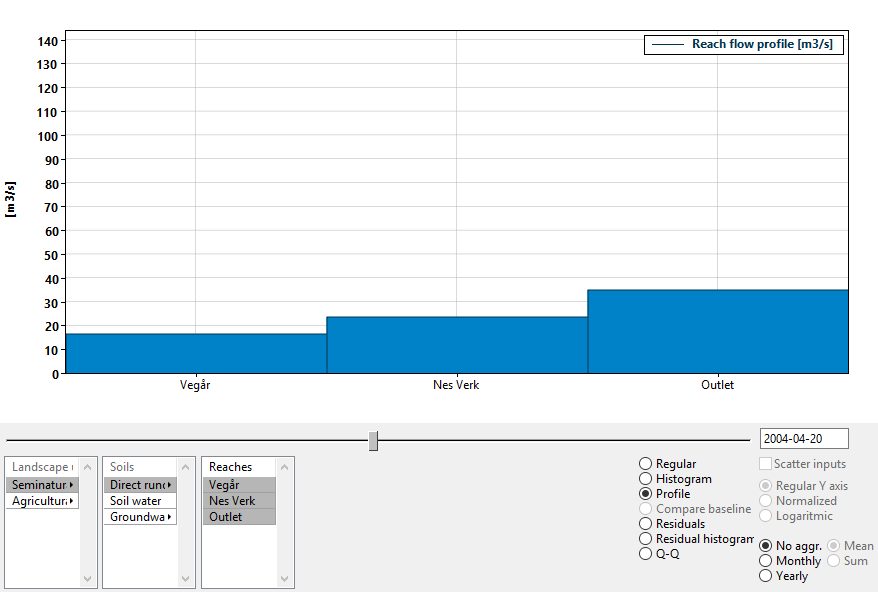
\includegraphics[width=0.7\linewidth]{img/scr2}
\captionof{figure}{When using the Profile plot mode you can select the date using a slider or a date text field.}
\end{center}

\subsubsection{Compare baseline}

This is only available if you have clicked the "Save baseline" button in the toolbar. You must have only one result time series (and optionally one input time series) selected. The plot will display both the current value of the selected time series and the value of the time series at the point you clicked "Save baseline". All plot options are available.

This can be useful for exploring differences in outcome between different parameter sets. For instance, you can see how it affects the stream nitrate concentration if you change the agricultural fertilizer nitrate input in INCA-N.

\subsubsection{Residuals}

You must have exactly one result time series and one input time series selected. The plots shows the residual time series (observed - modeled). Select "Scatter inputs" to display it as a scatter plot instead of a line plot.

To compare your modeled time series against an observed series, you can load the observed series in as an "additional timeseries", which is explained in the Mobius file format documentation.

A linear regression line of the residuals is also displayed. This shows the trend in the residuals. For instance if this trend goes up, it says that the observed quantity increases over time compared to the modeled one. The regression line is only computed for the GOF interval (see section \ref{sec:gofint}).

You can also use aggregation. For instance, the monthly sum of the residuals of something like "Reach flow" versus "Observed discharge" can tell you something about the monthly water balance in a hydrology model.

\subsubsection{Residual histogram}

You must have exactly one result time series and one input time series selected. The shows a histogram of the residuals. The number of bins are selected using the same rule as for the Histogram option. Moreover, red dots show what the distribution of residuals would look like if it was perfectly normally distributed (with the same mean and standard deviation).

\subsubsection{Q-Q}

You must have exactly one result time series and one input time series selected. This shows a quantile-quantile plot of the two time series, and can be used to see if your modeled time series is roughly similarly distributed to the observed one.

The displayed percentiles are 5, 15, 25, 50, 75, 85, 95. The X axis is the result series, while the Y axis is the input series. The two have the same quantiles if the blue dots are on the red diagonal line.

\subsection{Context menu options (edit or save plot)}

In addition to what we have implemented in MobiView (described above), the plot has all of the functionality of the ScatterCtrl package from the Ultimate++ framework. You can right click the plot to get a context menu, where you can
\begin{enumerate}[i]
\item Select zooming or panning options.
\item Edit text fields, select colors and plot styles (Properties).
\item Get a table of the underlying data of the plot (Data). Can e.g. be copied to Excel by selecting multiple cells and ctrl-C.
\item Copy the plot as an image to the clipboard (Copy image). This only works correctly if you want to paste into certain applications. It works with most image editing software, Microsoft applications (e.g. Word, Outlook, Internet Explorer), but sadly there is a bug right now where it does not work with the Google Chrome browser.
\item Save the image of the plot (Save image). Several formats are available (e.g. png, pdf).
\end{enumerate}

\subsection{The GOF interval}\label{sec:gofint}

If you have selected one of the Residual, Residual histogram or the Q-Q plot modes, you can select the GOF interval below the timseries info box. The interval consists of two dates, and only timesteps between these dates will be considered in the plot and in the goodness-of-fit computations (see next section).

\begin{center}
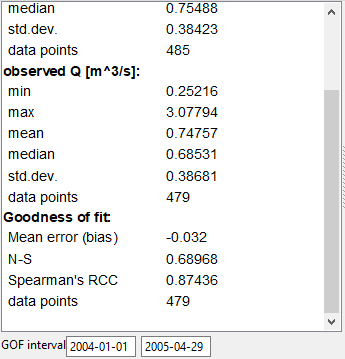
\includegraphics[width=0.3\linewidth]{img/scr3}
\captionof{figure}{When in a Residual-type plot mode, the GOF interval can be chosen using the two date text fields below the time series info box, where the goodness-of-fit stats are displayed.}
\end{center}

\subsection{Goodness-of-fit statistics}\label{sec:gof}

The goodness-of-fit statistics are displayed in the time series info box if you have exactly one result series and one input series selected, and have selected one of the Residuals, Residual histogram or Q-Q plot modes. 

Most of the goodness-of-fit statistics are implemented following \cite{krause05}. Further properties of the various statistics are discussed in that paper.

Let $o=\{o_i\}_{i\in I}$ be the observed time series, and let $m=\{m_i\}_{i\in I}$ be the modelled time series. The set $I$ of comparison points is the set of all timesteps in the GOF interval where both series have a valid value. For instance, the observed time series can have missing values, so the timesteps corresponding to the missing values will not be considered when evaluating goodness-of-fit. The GOF interval is the entire model run interval unless something else is specified by the user. Let
\[
\overline{m} = \frac{1}{|I|}\sum_{i\in I}m_i
\]
denote the mean of a time series.

\subsubsection{Common data points}
The common data points is the size of the set of comparison points $I$, denoted $|I|$.

\subsubsection{Mean error (bias)}
The mean error is
\[
\overline{o - m} = \overline{o} -\overline{m} =\frac{1}{|I|} \sum_{i\in I} (o_i - m_i)
\]
For fluxes or flows, the mean error is related to the discrepancy in mass balance.

\subsubsection{MAE}
MAE is the mean absolute error
\[
\frac{1}{|I|}\sum_{i\in I}|o_i - m_i|,
\]
where $|\cdot|$ denotes the absolute value of a number.

\subsubsection{RMSE}
RMSE is the root mean square error
\[
\sqrt{\frac{1}{|I|}\sum_{i\in I}(o_i-m_i)^2}.
\]

\subsubsection{N-S}
N-S is the Nash-Sutcliffe efficiency coefficient \cite{nashsutcliffe70}
\[
1 - \frac{\sum_{i\in I}(o_i - m_i)^2}{\sum_{i\in I}(o_i-\overline{o})^2}.
\]
This coefficient takes values in $(-\infty, 1]$, where a value of $1$ means a perfect fit, while a value of $0$ or less means that the modeled series is a no better fit than a series constantly equal to the mean of the observed series.

\subsubsection{log N-S}
log N-S is the same as N-S, but where $o_i$ is replaced by $\ln(o_i)$ and $m_i$ replaced by $\ln(m_i)$ for each $i\in I$. Here $\ln$ denotes the natural logarithm.
\[
1 - \frac{\sum_{i\in I}(\ln(o_i) - \ln(m_i))^2}{\sum_{i\in I}(\ln(o_i)-\overline{\ln(o)})^2}.
\]
This coefficient behaves similarly to N-S, but is less sensitive to errors on time steps where both series have large values.

\subsubsection{r2}
$r^2$ is the coefficient of determination
\[
\left(\frac{\sum_{i\in I}(o_i-\overline{o})(m_i-\overline{m})}{\sqrt{\sum_{i\in I}(o_i-\overline{o})^2}\sqrt{\sum_{i\in I}(m_i-\overline{m})^2}}\right)^2.
\]
This coefficient takes values in $[0, 1]$.

\subsubsection{Idx. of agr.}
The index of agreement is
\[
1 - \frac{\sum_{i\in I}(o_i-m_i)^2}{\sum_{i\in I}(|m_i-\overline{o}| + |o_i-\overline{o}|)^2}.
\]

\subsubsection{KGE}
KGE is the Kling-Gupta efficiency \cite{klinggupta09}
\[
1 - \sqrt{(r-1)^2 + (\beta-1)^2 + (\delta-1)^2}
\]
where $r$ is the square root of the coefficient of determination $r^2$, $\beta=\overline{m}/\overline{o}$, and $\delta=Cv(m)/Cv(o)$, $Cv(x)=\sigma(x)/\overline{x}$, $\sigma$ being the standard deviation.

\subsubsection{Spearman's RCC}
Spearman's rank correlation coefficient \cite{spearman04} is computed as follows: For a time series $x=\{x_i\}_{i\in_I}$, let $\mathrm{rank}(x_i)$ be the index of $x_i$ (starting from 1) in the list $\mathrm{sort}(x)$, where $\mathrm{sort}(x)$ is $x$ sorted from smallest to largest. The rank correlation coefficient can then be computed as
\[
1 - \frac{6\sum_{i\in I}(\mathrm{rank}(o_i)-\mathrm{rank}(m_i))^2}{|I|(|I|^2 - 1)}.
\]
The coefficient takes values in $[-1, 1]$. If the value is 1, the modeled series is a (positively) monotone function of the observed series.


\bibliographystyle{plain}
\bibliography{citations}

\end{document}